%Fazer um merge das duas últimas sessẽos para uma única mais simplificadamente.

%<apresentar uma pequena descrição dos assuntos apresentados nas sub-seções seguintes>%
%<Um ultimo paragrafo ligando estes quatro temas, sem ainda dizer o que você vai fazer>%
\section{REFERENCIAL BIBLIOGRÁFICO}
Esta seção, apresenta as principais referências que contextualizam este trabalho. A subseção 2.1 descreve sobre Arquitetura de Software. A subseção 2.2 descreve Visão Arquitetural. A subseção 2.3 resume Sistemas de Informação. Já a subseção 2.4 apresenta Arquitetura de Referência para Sistemas de Informação. A subseção 2.5 apresenta de forma geral Arquiteturas de Aplicativos Móveis. A subseção 2.6 faz uma breve revisão sobre Projetos de Aplicativos Móveis. A subseção 2.7 faz uma breve revisão sobre tecnologias suportadas na arquitetura deste trabalho: \textit{web services}, o estilo arquitetural \textit{REST}, o \textit{Push Notification} e o JSON. Para finalizar, a subseção 2.8 destaca sobre Desenvolvimento de Software Orientado a Componentes.


%<dizer os benefícios em trabalhar orientado a arquiteturas: controle intelectual, atendimento de requisitos não-funcionais, evolução, \textit{testability}, etc>%
%<dizer como as arquiteturas são projetadas>%
%<cada domínio de aplicação em particular demanda a adoção de arquiteturas particulares>%
\subsection{Arquitetura de Software}
De acordo com a definição clássica proposta por \textit{Shaw e Garlan} \cite{shaw_and_garlan}, arquitetura de software define o que é sistema em termos de componentes computacionais e os relacionamentos entre eles, os padrões que guiam suas composições e restrições. Arquitetura de software pode ser compreendida como uma especificação abstrata do funcionamento de um sistema e permite especificar, visualizar e documentar a estrutura e o funcionamento de um programa independente da linguagem de programação na qual ele será implementado \cite{jair_Cavalcanti_leite}.\par

Os softwares estão em constante evolução e sofrem mudanças periodicamente, que ocorrem por necessidade de corrigir \textit{bugs} ou de adicionar novas funcionalidades. As mudanças ocorridas no processo de evolução de um software podem torná-lo instável e predisposto a defeitos, além de causar atraso na entrega e custos acima do estimado. Porém, um software que é projetado orientado a arquitetura, possibilita os seguintes benefícios:
\begin{enumerate}
		\item Melhor escalabilidade;
		\item Maior controle intelectual;
		\item Menor impacto causado pelas mudanças;
		\item Melhor atendimento aos requisitos não-funcionais;
		\item Maior agilidade na manutenção do código;
		\item Padronização de comunicação entre os componentes e;
		\item Suporte a reuso dos componentes e maior controle dos mesmos.
\end{enumerate}

O desenvolvimento de software envolve muitas partes (e.g., levantamento de requisitos, modelagem, implementação, testes, refatoração e etc.). O objetivo de um software é o que motiva a sua construção, e o que fomenta todas as partes que envolve o seu desenvolvimento é o problema que ele tenta solucionar no mundo real e parte do mérito de uma boa solução é devido ao uso de uma boa arquitetura.

Neste trabalho, arquitetura de software pode ser compreendida nas decisões de implementação, nas restrições impostas pelo uso dos recursos disponibilizados e dos componentes reutilizáveis, além dos estilos arquiteturais provenientes das APIs utilizadas, tais como, o \textit{Event-Based}, mecanismo de comunicação orientado a eventos provido pelo Qt/QML e o \textit{Restful} que é utilizado como \textit{web service} suportado pela aplicação. Outro aspecto arquitetural deste trabalho é um estilo de desenvolvimento orientado a plugins que constituem os componentes específicos de cada projeto ou aplicação baseada nesta arquitetura. Os plugins formarão os principais recursos do sistema e são independentes entre si. O principal destaque em uma arquitetura de plugins é o baixo acoplamento entre as funcionalidades do sistema.


\subsection{Visão Arquitetural}
A arquitetura de um software pode ser representada de vários pontos de vista, que podem ser combinados para criar uma visão holística do sistema \cite{guideline:architectural_view}. As visões arquiteturais são diferentes formas de observar a arquitetura de um software, cada qual ressaltando aspectos específicos e relevantes conforme o papel da pessoa que está definindo a arquitetura e a etapa do processo de desenvolvimento em que ela se encontra \cite{Raymond1995}. Os requisitos funcionais implementados nesta arquitetura serão apresentados em um tópico seguinte em visões arquiteturais através de imagens e diagramas da UML. O objetivo das visões é facilitar a compreensão das partes que compõe esta arquitetura.


\subsection{Sistemas de Informação}
Um sistema de informação pode ser definido como um conjunto de componentes inter-relacionados trabalhando juntos para coletar, recuperar, processar, armazenar e distribuir informações com a finalidade de facilitar o planejamento, o controle, a coordenação, a análise e o processo decisório em organizações \cite{laudon}.


\subsection{Arquitetura de Referência para Sistemas de Informação}
Uma arquitetura de referência consiste em uma forma de apresentar um padrão genérico para um projeto \cite{zambiasi}. Com base nessa arquitetura, o desenvolvedor projeta, desenvolve e configura uma aplicação prototipando-a por meio de componentes reutilizáveis \cite{zambiasi}.\par

Para compor uma arquitetura de referência é necessário apresentar os tipos dos elementos envolvidos, como eles interagem e o mapeamento das funcionalidades para estes elementos \cite{Hofmeister:1999:ASA:322640}. De maneira geral, uma arquitetura de referência deve abordar os requisitos para o desenvolvimento de soluções, guiado pelo modelo de referência e por um estilo arquitetural de forma a atender as necessidades do projeto \cite{c._k_f._2006}. A concepção de uma arquitetura de referência pode ser entendida neste trabalho como uma forma de disponibilizar um padrão genérico para o desenvolvimento de novos aplicativos no contexto de sistemas de informação.\par

O domínio de aplicações móveis engloba vários requisitos e restrições que variam entre limitações de hardware tais como energia limitada, baixo poder de processamento e limitação de recursos como armazenamento e realizar comunicação remota quando o dispositivo está em rede móvel. Ao utilizar uma arquitetura de referência, é possível obter recursos implementados para funcionalidades corriqueiras no contexto da aplicação, como persistir dados, obter informações de um \textit{web service}, exibir uma notificação para o usuário e etc.


\subsection{Arquiteturas de Aplicativos Mobile}
Arquitetura para aplicações móveis abrange quatro camadas: Interação Humana-Computador (\textit{IHC}), Aplicação Móvel, \textit{Middleware} e \textit{Enterprise Backend} \cite{Pabllo:2008:MMA:1621087.1621128}. Neste trabalho, a arquitetura foi concentrada apenas nas camadas de interação, aplicação e \textit{Middleware}.

\subsubsection{Camada de Interação Humana-Computador}
A camada de Interação Humana-Computador (mais conhecida como interface de usuário, ou simplesmente UI) define os elementos de interação entre o usuário e os recursos do aplicativo. De forma abstrata, a camada de interface do usuário descreve o tipo de mídia suportada pelo aplicativo (por exemplo, texto, gráficos, imagens, vídeo ou som), os tipos de mecanismos de entrada (por exemplo, teclado alfa-numérico, ponteiros de caneta ou toques na tela) e os tipos de mecanismos de saída (por exemplo, uma notificação na bandeja do sistema, a tela, os alto-falantes ou algum tipo de \textit{feedback} como vibrar o dispositivo) \cite{Pabllo:2008:MMA:1621087.1621128}. Um exemplo de um componente desta camada é o objeto \textit{Image} do QML que corresponde ao carregamento e exibição de uma imagem na tela, além de botões, campos de texto e elementos que suportam cliques.

\subsubsection{Camada de aplicação}
A camada de aplicação corresponde ao processamento de ações e eventos provenientes da camada de interação, como por exemplo, captando eventos de toque em objetos visuais e realizando processamento em segundo plano como trocar a página atualmente vista pelo usuário, utilizando algum parâmetro lido em um objeto \textit{JSON}. Esta camada, corresponde a componentes não visuais e interagem diretamente com a camada de \textit{middleware}. Objetos da camada de aplicação podem por exemplo, gerenciar e controlar a criação de outros componentes tais como, o objeto \textit{StackView} do QML, que instancia páginas dinamicamente a partir de cliques em um menu de opções.

\subsubsection{Camada de middleware}
A camada de \textit{middleware} intercala entre a camada de aplicação com a camada de \textit{backend}. O objetivo dessa camada é fornecer de forma abstrata e genérica um meio de comunicação entre o modelo de dados da aplicação com a camada de \textit{backend} \cite{Pabllo:2008:MMA:1621087.1621128}. Ela é também responsável por interagir com o meio de comunicação disponível no dispositivo abstraindo para a camada de aplicação qual foi a interface de hardware utilizada. Objetos da camada de \textit{middleware} podem ser executados de forma assíncrona para que não bloqueiem os eventos da tela, enquanto aguardam um feedback da camada de \textit{backend} para permitir melhor desempenho e usabilidade da aplicação. Exemplos de componentes dessa camada são objetos que realizam acesso a rede através de requisições HTTP.

\subsubsection{Camada de backend}
A camada \textit{backend} consiste de uma outra aplicação que responde pelas requisições do aplicativo através de uma rede via protocolo \textit{HTTP}. Esta camada está associada ao \textit{web service} ou serviço REST. O \textit{web service} pode atender a diferentes requisições e dispositivos, além de abstrair para a aplicação, toda lógica de negócios referente ao armazenamento e processamento dos dados do sistema. A implementação desta camada pode ser desenvolvida sobre uma outra arquitetura, além de implementar regras de negócio inerentes ao seu funcionamento.

%caberia aqui uma imagem que mostrasse o relacionamento/interação entre essas 4 camadas!%



%<definir o que é um aplicativo móvel: de onde surgiu esse termo? Porque aplicativo e não aplicação ou mesmo software?>%
%<porque o uso tão popular dos aplicativos moveis?>%
%<características particulares dos aplicativos móveis.O que fazem eles diferentes das aplicações web, desktop, em cloud, etc?>%
%<demandas arquiteturais trazidas pelos aplicativos móveis>%
\subsection{Projeto de Aplicativos Móveis}
Um projeto é um esforço temporário empreendido para criar um produto, serviço ou resultado exclusivo. O termo temporário quer dizer que o projeto possui um ciclo de vida com início e final determinados \cite{governanadetidotcom}. O projeto termina quando seus objetivos forem alcançados ou quando existirem motivos para não continuá-lo \cite{governanadetidotcom}. Um aplicativo móvel ou aplicação móvel ou simplesmente \textit{app}, é um sistema desenvolvido para ser instalado e executado em um dispositivo eletrônico portátil, como tablets e smartphones \cite{what_is_mobile}.\par

Um aplicativo móvel pode ser baixado diretamente no aparelho eletrônico, desde que o dispositivo possua conexão com a Internet. O mercado de dispositivos móveis é ramificado por diferentes fabricantes, o que inclui uma variação de plataformas de desenvolvimento, sistemas operacionais, versões do SO e configuração variada de hardware. Na construção de um aplicativo para dispositivo móvel, a implementação é um ponto muito importante, pois, além de representar a parte concreta dos requisitos funcionais do aplicativo também refletem diretamente nos requisitos não funcionais e consequentemente na qualidade do software.\par

O sucesso de aplicativos para dispositivos móveis vai além das medidas de desempenho, portabilidade e usabilidade tradicionais \cite{Kronbauer:2012:UEE:2393536.2393582}. Os aplicativos devem estar em conformidade com a personalidade, preferências, objetivos, experiências e conhecimento de seus usuários \cite{Vermeeren:2010:UEE:1868914.1868973}. Além disso, o contexto físico, social e virtual onde ocorrem as interações deve, sempre que possível, ser levado em consideração \cite{McCarthy:2004:TE:1015530.1015549}.\par

Torna-se evidente que são muitos requisitos a serem considerados em um projeto de aplicativo móvel. O esforço dedicado para atender a todos os requisitos pode tornar o projeto enfadonho, além de exigir tempo e mão de obra. O processo de desenvolvimento pode ser otimizado através de ferramentas como \textit{frameworks} ou uma arquitetura de componentes reutilizáveis, a fim de agilizar e auxiliar o processo de desenvolvimento.


\subsection{Desenvolvimento de Software Orientado a Componentes}
O desenvolvimento de software Orientado a componentes é um paradigma da engenharia de software caracterizado pela composição de partes já existentes, ou desenvolvidas independentemente e que são integradas para atingir um objetivo final \cite{rafael_heider}. Construir novas soluções pela combinação de componentes desenvolvidos aumenta a qualidade e dá suporte ao rápido desenvolvimento, levando à diminuição do tempo de entrega do produto final ao mercado \cite{rafael_heider}. Os sistemas definidos através da composição de componentes permitem que sejam adicionadas, removidas e substituídas partes do sistema sem a necessidade de sua completa substituição. Com isso, o desenvolvimento baseado em componentes auxilia na manutenção do software, por permitir que o sistema seja atualizado através da integração de novos componentes ou atualização dos objetos já existentes \cite{szyperski_bosch_weck_1999}.\par

O reuso de componentes é um recurso extra da arquitetura apresentada neste trabalho, pois dispõe de trinta componentes (visuais e não visuais) reutilizáveis para auxiliar no desenvolvimento de novos aplicativos, seguindo as restrições desta arquitetura que é dedicada a sistemas de informação. Estes componentes são arquivos QML genéricos que podem atender a diferentes customizações através das propriedades disponibilizadas pelos seus elementos internos, que permitem definir ou alterar os valores pre-definidos. Os benefícios da componentização estão ligados a manutenibilidade, reúso, composição, extensibilidade, integração e escalabilidade \cite{D'Souza:1998:OCF:291139}.\par


%<introducao aos servicos web>%
%<tecnologias para servicos web: SOAP, RESTful, etc>%
%<definir o que é o RESTful>%
%<colocar uma figura explicando uma requisicao RESTful convencional>%
%<benefícios do RESTful: porque tem sido amplamente adotado?>%
\subsection{Web Services, RESTful, Push Notification e JSON}
Os \textit{web services} constituem uma tecnologia emergente da Arquitetura Orientada a Serviços (SOA) \cite{perepletchikov}. Com a expansão da internet e a necessidade de integração entre aplicações web, tornou-se necessário a centralização de informações para serem acessados por diferentes clientes. Para esse propósito, foi criada a tecnologia de \textit{web services} \cite{ibm_research}. Uma característica fundamental dos \textit{web services}, diz respeito à possibilidade de utilização de diferentes formas de transmissão de dados pela rede e o atendimento a diferentes clientes e dispositivos. Logo, a arquitetura de \textit{web services} pode trabalhar com protocolos HTTP, SMTP, FTP, RMI ou protocolos de mensagem proprietários.\par

o RESTFul é um estilo arquitetural para a construção de sistemas distribuídos \cite{fielding}. O elemento fundamental da arquitetura RESTful é o \textit{resource} ou recurso. Um recurso pode ser uma página web contendo um documento estruturado, uma imagem ou até mesmo um vídeo. Para localizar os recursos envolvidos em uma interação entre os componentes da arquitetura RESTful é utilizado o chamado identificador de recurso ou \textit{URI}. Com isso, um recurso pode ser representado através de diferentes formatos e o mais comum e utilizado é o \textit{JSON}. O termo REST, é empregado em serviços RESTful que não implementam todos os princípios da especificação do estilo arquitetural definido por \textit{Fielding} \cite{fielding}. Para que todos os princípios deste estilo sejam respeitados, um conjunto de restrições deve ser seguido, os quais não serão abordados neste trabalho. Para facilitar a compreensão geral de um serviço REST, a imagem à seguir foi adicionada para representar um modelo de comunicação entre um cliente ou dispositivo e um serviço RESTful.

\begin{figure}[h]
	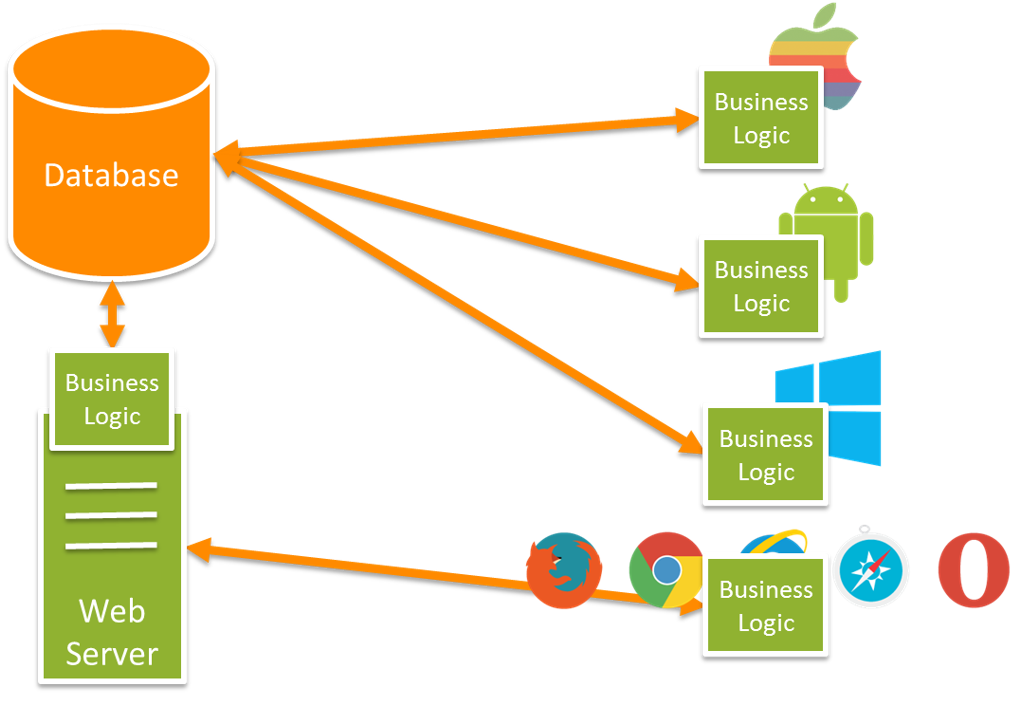
\includegraphics[width=8cm]{restful_request}
	\centering
	\caption{Processo de comunicação de um serviço REST}
\end{figure}

\textit{Push Notification} é descrito por Acer et al. \cite{Acer:2015:EES:2902314.2902344} como mensagens pequenas, usadas por aplicações de celular para informar aos usuários sobre novos eventos e atualizações. As notificações na maioria dos casos, estão associadas aos aplicativos instalados no dispositivo. O termo \textit{push} indica que a mensagem parte do servidor para o dispositivo. Os principais provedores de notificações via \textit{push} são o \textit{Apple Push Notification Server} (APN) e o \textit{Firebase} antigo \textit{Google Cloud Messaging}. A imagem à seguir, apresenta o modelo de comunicação que ocorre no envio de um \textit{Push Notification}.\par

\begin{figure}[h]
	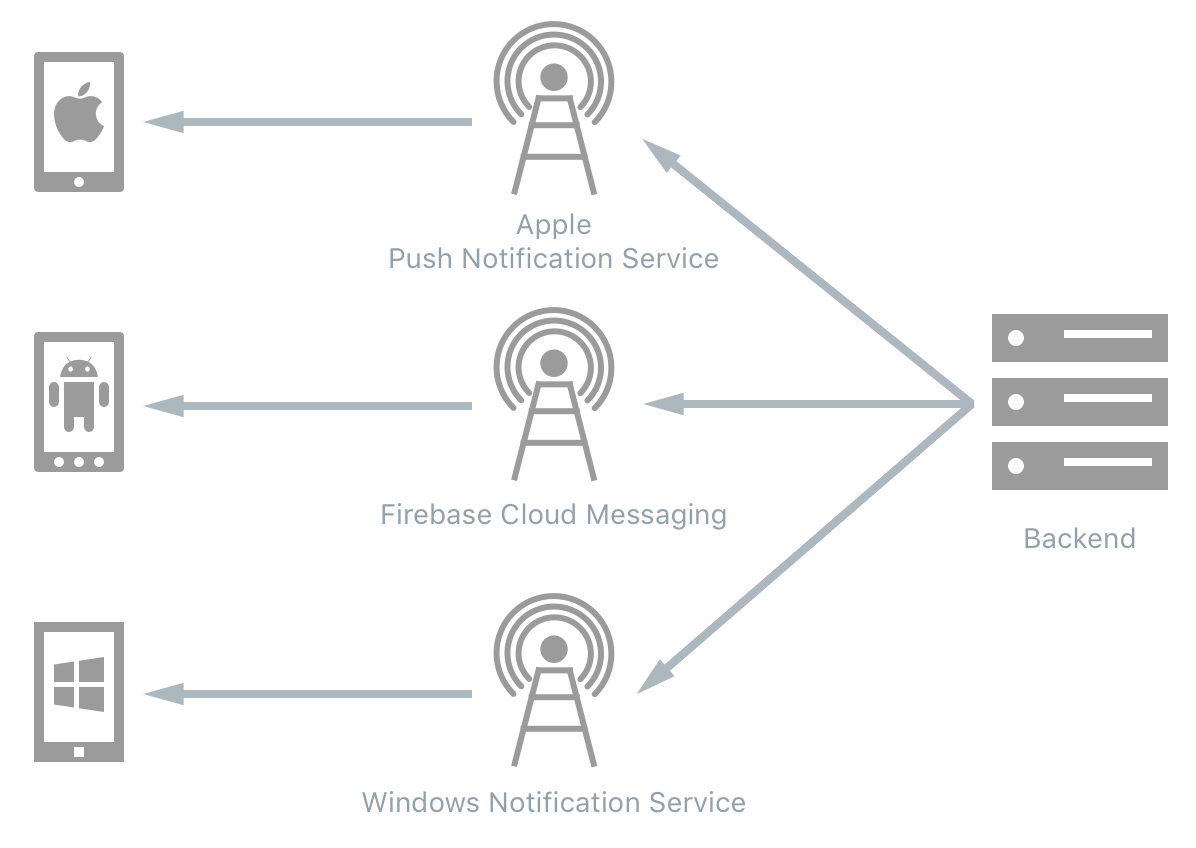
\includegraphics[width=8cm]{push_notification}
	\centering
	\caption{Processo de comunicação de um \textit{push notification}}
\end{figure}

O JSON\footnote{https://json.org} (\textit{JavaScript Object Notation}) é um conjunto de chaves e valores, que podem
ser interpretados por qualquer linguagem. Além de ser um formato de troca de dados largamente utilizado em serviços REST, é fácil de ser entendido e escrito pelos programadores. Estas propriedades fazem do JSON um objeto ideal para o intercâmbio de dados em aplicações web tal como o XML \cite{jun_y_zhishu}.